%%%%%%%%%%%%%%%%%%%%%%%%%%%%%%%%%%%%%%%%%%%%%%%%%%%%%%%%%%%%
% Preamble:
%%%%%%%%%%%%%%%%%%%%%%%%%%%%%%%%%%%%%%%%%%%%%%%%%%%%%%%%%%%%

% automatically loads e.g.
%   xcolor
%   colortbl - commands for colorizing tables
%   hyperref - e.g. \url, \href, inter-PDF-links ...
\documentclass[xcolor={dvipsnames,table}]{beamer}

\mode<presentation>
{
  \usetheme{Hannover}

  % innercolor theme
  \usecolortheme{orchid}
  % outer color theme
  \usecolortheme{whale}
}

\usepackage[utf8]{inputenc}
\usepackage[T1]{fontenc}
% latin modern - 'The fonts, as compared to the CM family,
% contain a lot of additional characters, mainly accented
% ones.' http://www.ctan.org/tex-archive/fonts/lm/
\usepackage{lmodern}

\usepackage[english]{babel}
%\usepackage[ngerman]{babel}

% e.g.: \includegraphics ...
\usepackage{graphicx}

% e.g. \align ...
\usepackage{amsmath}

% verbatim program code:
\usepackage{listings}
\lstset{language=C,
  basicstyle=\ttfamily,
  commentstyle=\color{ForestGreen}
}

% nicer tables:
% \usepackage{booktabs}

\institute{Universität Bielefeld}
\title{Title}
\subtitle{Subtitle}
\author{Joe User}
%\date{}
%\logo{}


%%%%%%%%%%%%%%%%%%%%%%%%%%%%%%%%%%%%%%%%%%%%%%%%%%%%%%%%%%%%
% Document:
%%%%%%%%%%%%%%%%%%%%%%%%%%%%%%%%%%%%%%%%%%%%%%%%%%%%%%%%%%%%

\begin{document}

\begin{frame}
\titlepage
\end{frame}

\section{Introduction}

\begin{frame}{Introduction}
  Lorem ipsum dolor sit amet, consectetur adipisicing elit, sed
  do eiusmod tempor incididunt ut labore et dolore magna aliqua.
  Ut enim ad minim veniam, quis nostrud exercitation ullamco
  laboris nisi ut aliquip ex ea commodo consequat.
\end{frame}

  \subsection{Overview}

  \begin{frame}{Overview}
    \begin{itemize}
      \item eiusmod
      \item tempor
      \item incididunt
    \end{itemize}
    \begin{block}{Important}
      \begin{enumerate}
        \item dolore
        \item magna
        \item aliqua
      \end{enumerate}
    \end{block}
  \end{frame}

\section{Results}

\begin{frame}
  \frametitle{Results}
  \begin{columns}
    \begin{column}{0.6\textwidth}
      Duis aute irure dolor in reprehenderit in voluptate velit
      esse cillum dolore eu fugiat nulla pariatur. Excepteur sint
      occaecat cupidatat non proident, sunt in culpa qui officia
      deserunt mollit anim id est laborum.
    \end{column}
    \begin{column}{0.4\textwidth}
      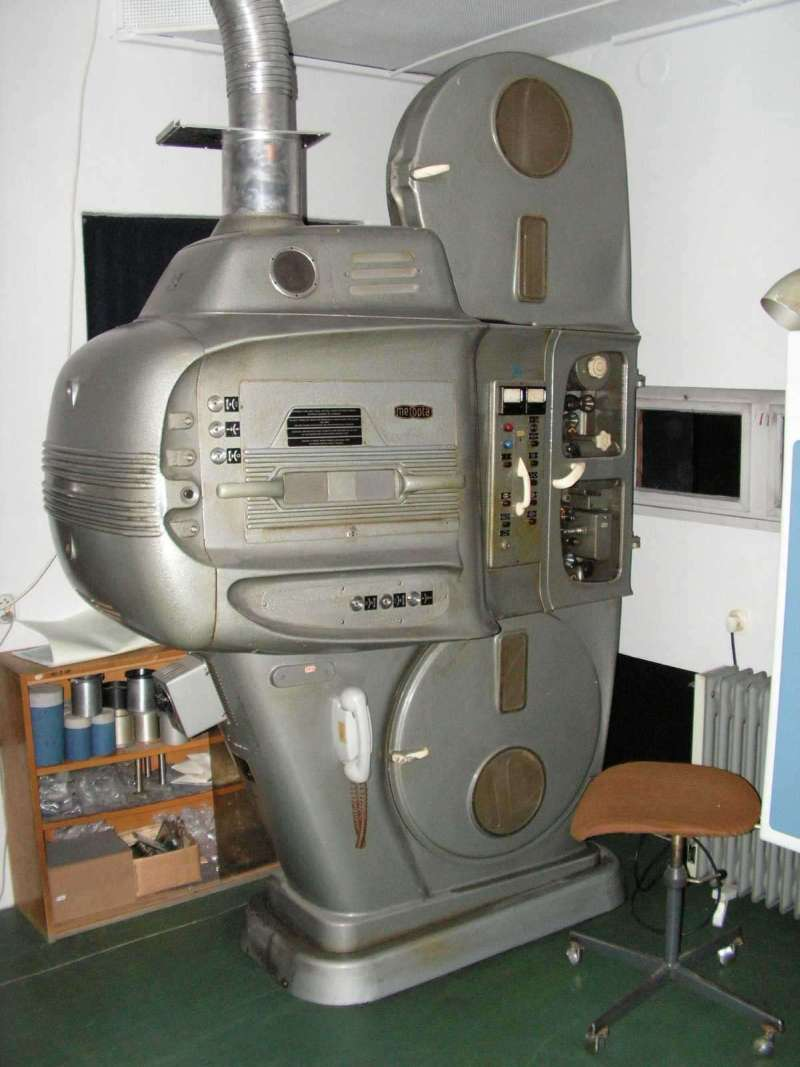
\includegraphics[width=1\textwidth]{Meopton_UM70x35_69118.jpg}
    \end{column}
  \end{columns}
  \begin{flushright}
    { \tiny Image: Public Domain,
      \url{http://commons.wikimedia.org/wiki/File:Meopton_UM70x35_69118.jpg}
    }
  \end{flushright}
\end{frame}

  \subsection{Overlays}

  \begin{frame}{Pause}
    \begin{example}
      \begin{equation}
        a + b \geq c
      \end{equation}
    \end{example}
    \pause
    \begin{block}{Block}
      \begin{itemize}
        \item 1
          \pause
        \item 2
        \item 3
      \end{itemize}
    \end{block}
  \end{frame}

  \begin{frame}{Overlay Specifications}
    \begin{itemize}
      \item<2-3> only on slides 2 to 3
      \item<1-> on every slide
    \end{itemize}
    \begin{block}{Warning}<2->
      \alert{Don't over-use overlays \dots}
    \end{block}
    \vspace{3em}
    \begin{onlyenv}<4->
      $\Rightarrow$ see Beamer Userguide (Section 9) for a reference on overlay
      specifications, commands and environments
    \end{onlyenv}
  \end{frame}

\section{Conclusion}

\begin{frame}[fragile]{Conclusion}
  \begin{lstlisting}
// Is this program correct?
int main()
{
  char *s;
  strcpy(s, "Hello World");
  puts(s);
  return 0;
}
\end{lstlisting}
\end{frame}

\begin{frame}{Color-Table}
\rowcolors{2}{BurntOrange}{YellowOrange}
\begin{tabular}{ll}
  \rowcolor{black}
  \color{white} Sprache & \color{white} \#Keywords \\
 Haskell &  21 \\
 Scheme &  23 \\
 C (C89) &  32 \\
 Java &  50 \\
 Ada &  72 \\
 C++ &  74 \\
\end{tabular}
\end{frame}

\end{document}
